%detector
\section{A Simple Probabilistic Detector}
Consider a system of $N$ sensors that are identical and detect an
event of time period $\tau$ such as a gunshot or an explosion. Let
the probability that an event $E$ has occurred, given that the
sensor measurement $s_i$ exceeds a threshold $T$ be given as:
\begin{equation}
P(E|s_i>T)=p \forall i\label{eqn:detrate},
\end{equation}
where $i=1\ldots N$ goes over all the sensors, and $0<p\leq 1$.
Similarly, let the probability of threshold crossing when the
event has not occurred, $E^c$ be given as:
\begin{equation}
P(E^c|s_i>T)=q \forall i\label{eqn:fprate},
\end{equation}
and $0<q\leq 1$. Let the number of samples produced by a sensor in
the course of the event equal $M=\lfloor \tau f_s \rfloor$, where
$f_s$ is the sampling frequency of all the sensors. Considering
the probabilities identical for all of the sensors is realistic if
the sensors respond to low frequency acoustics or thermal
radiation signature, which does not attenuate very much with
distance. Furthermore, we can also assume that the detection is at
the same instant for all of the sensors if the sensors are not
separated by distances larger than the signal would travel in a
sampling interval (e.g., for an acoustic sensor system $10$ms or
$100$Hz sampling gives around $3$ meters separation for the
sensors).

Now consider a detection function defined as follows that combines
data from all of the sensors to detect an event and determine its
time:
\begin{eqnarray}
% \nonumber to remove numbering (before each equation)
  f &=& {1\over MN}\sum_{i=1}^{MN}d_i\label{eqn:detector} \\
  d_i &=&\left\{\begin{array}{lr}
  1 & s_i>T\\
  0 & {\rm otherwise}\end{array}\right.
\end{eqnarray}

The relevant questions that can be asked at this point are--
\begin{itemize}
\item What is the expected value of $f$ if an event occurs? \item
What is the expected value of $f$ if the event does not occur?
\end{itemize}
If there are no bandwidth limitations and there is perfect time
synchronization between the sensors, we will have
\begin{eqnarray}
% \nonumber to remove numbering (before each equation)
  E\langle f|E\rangle &=& p \nonumber\\
E\langle f|E^c\rangle   &=& q\label{eqn:perfectsync}.
\end{eqnarray}
The detection rate will be smaller and the false positive rate will be higher if there are bandwidth limits
and synchronization is not perfect if we threshold the detection function $f$ at the value $p$.

\subsection{Detection Rate under Synchronization Error}
Let us consider the detection system when the different sensors have different detection probabilities $p_i$ and different false positive probabilities $q_i$. The detection function can be expressed as
\begin{eqnarray}
% \nonumber to remove numbering (before each equation)
  f &=& {1\over N}\sum_{i=1}^Md_i \nonumber\\
  d_i &=& {1\over M}\sum_{k=1}^Md_{i,k}\label{eqn:heterog_detector}\\
  d_{i,k}&=& \left\{\begin{array}{lr}
  1 & s_{i,k}>T_i\\
  0 & {\rm otherwise}\end{array}\right.\nonumber
\end{eqnarray}
We can set thresholds using standard Bayesian methods if we know the distributions of noise in the different sensors along with the signal levels produced by the events. To consider the effect of synchronization error on the detector, let us assume that it follows a uniform distribution over the interval $[0,t_s]$ or almost equivalently, $[0,L]$, where $L=\lfloor t_sf_s\rfloor$, and that this distribution is identical for all the sensors. Now the probability that the sample of length $MN$ from which $f$ is computed was not produced in the interval $[t-\tau,t]$, or in the sampled case, $[k-M,k]$ can be calculated. We examine the most probable case that the event occurs in the interval $[k-M,k]$, and there is no event in the preceding interval. We assume that all detection results from individual sensors are transmitted to the node which produces $f$--we later generalize to the case where some of the bits are lost in transmission. Consider a sample received at time $l$ in the interval $[k-M,k]$. The probability that it came from a sensor before the event started is
\begin{equation}
% \nonumber to remove numbering (before each equation)
  p_{se,l} = \left\{\begin{array}{lr}
  {L-(l-k+M) \over L}  & L-M+k-l\geq 0\\
  0 & {\rm otherwise}\end{array}\right.\label{eqn:syncerrorprob},
\end{equation}
and the probability that it came from during the event is $1-p_{se,l}$. Without loss of generality, we can take $k=M$ or any multiple of it, so that $l$ goes from $0$ to $M$. Hence, the expected value of the composite detector $f$ can be calculated from the individual values of the $d_{i,l}$ as follows:
\begin{eqnarray}
% \nonumber to remove numbering (before each equation)
  E\langle f\rangle &=& {1\over N}\sum_{i=1}^N\langle d_i \rangle\nonumber\\
  \langle d_i \rangle&=& {1\over M}\sum_{l=1}^M p_i(1-p_{se,l})+q_ip_{se,l}\nonumber\\
  &=& p_i\left( {M+1 \over 2L}\right)+q_i\left(1- {M+1 \over 2L}\right)\label{eqn:heterog_detector_mean}
\end{eqnarray}
We can use these calculations in conjunction with the distributions
in~\cite{timing-error} to obtain realistic detector performance.\\

Figure \ref{fig:detection} shows the detection probability $E\langle
f\rangle$ with time synchronization error bound of 1ms and 1s drawn
in solid and dotted line respectively. Here, we assume that $p_i$ =
0.9 and $q_i$ = 0.05 with 10 randomly deployed sensors. The event
duration is 1 second for the analysis. In the figure, we can observe
two important results. First, the impact of timing error on
detection probability is significant. If the timing error is bounded
within 1 second, the detection probability is considerably lowered
compared to the case where timing error is bounded within 1ms. Thus,
reasonable timing error bounds are mandatory to achieve a good QoI.
Secondly, the application QoI is not linearly improved with sampling
rate. It shows a tendency that the detection probability is slightly
impaired with 2 $\sim$ 5 samples in the event duration period (0.5
$\sim$ 0.2 sampling frequency with 1 second event duration).
Opposite to our intuition that the detection probability would be
improved as the sampling rate increases, the sampling rate or
sampling frequency has minimal impact on detection application's
QoI. Rather, the limit of timing error plays more critical role in
terms of QoI.

\begin{figure}
    \begin{center}

    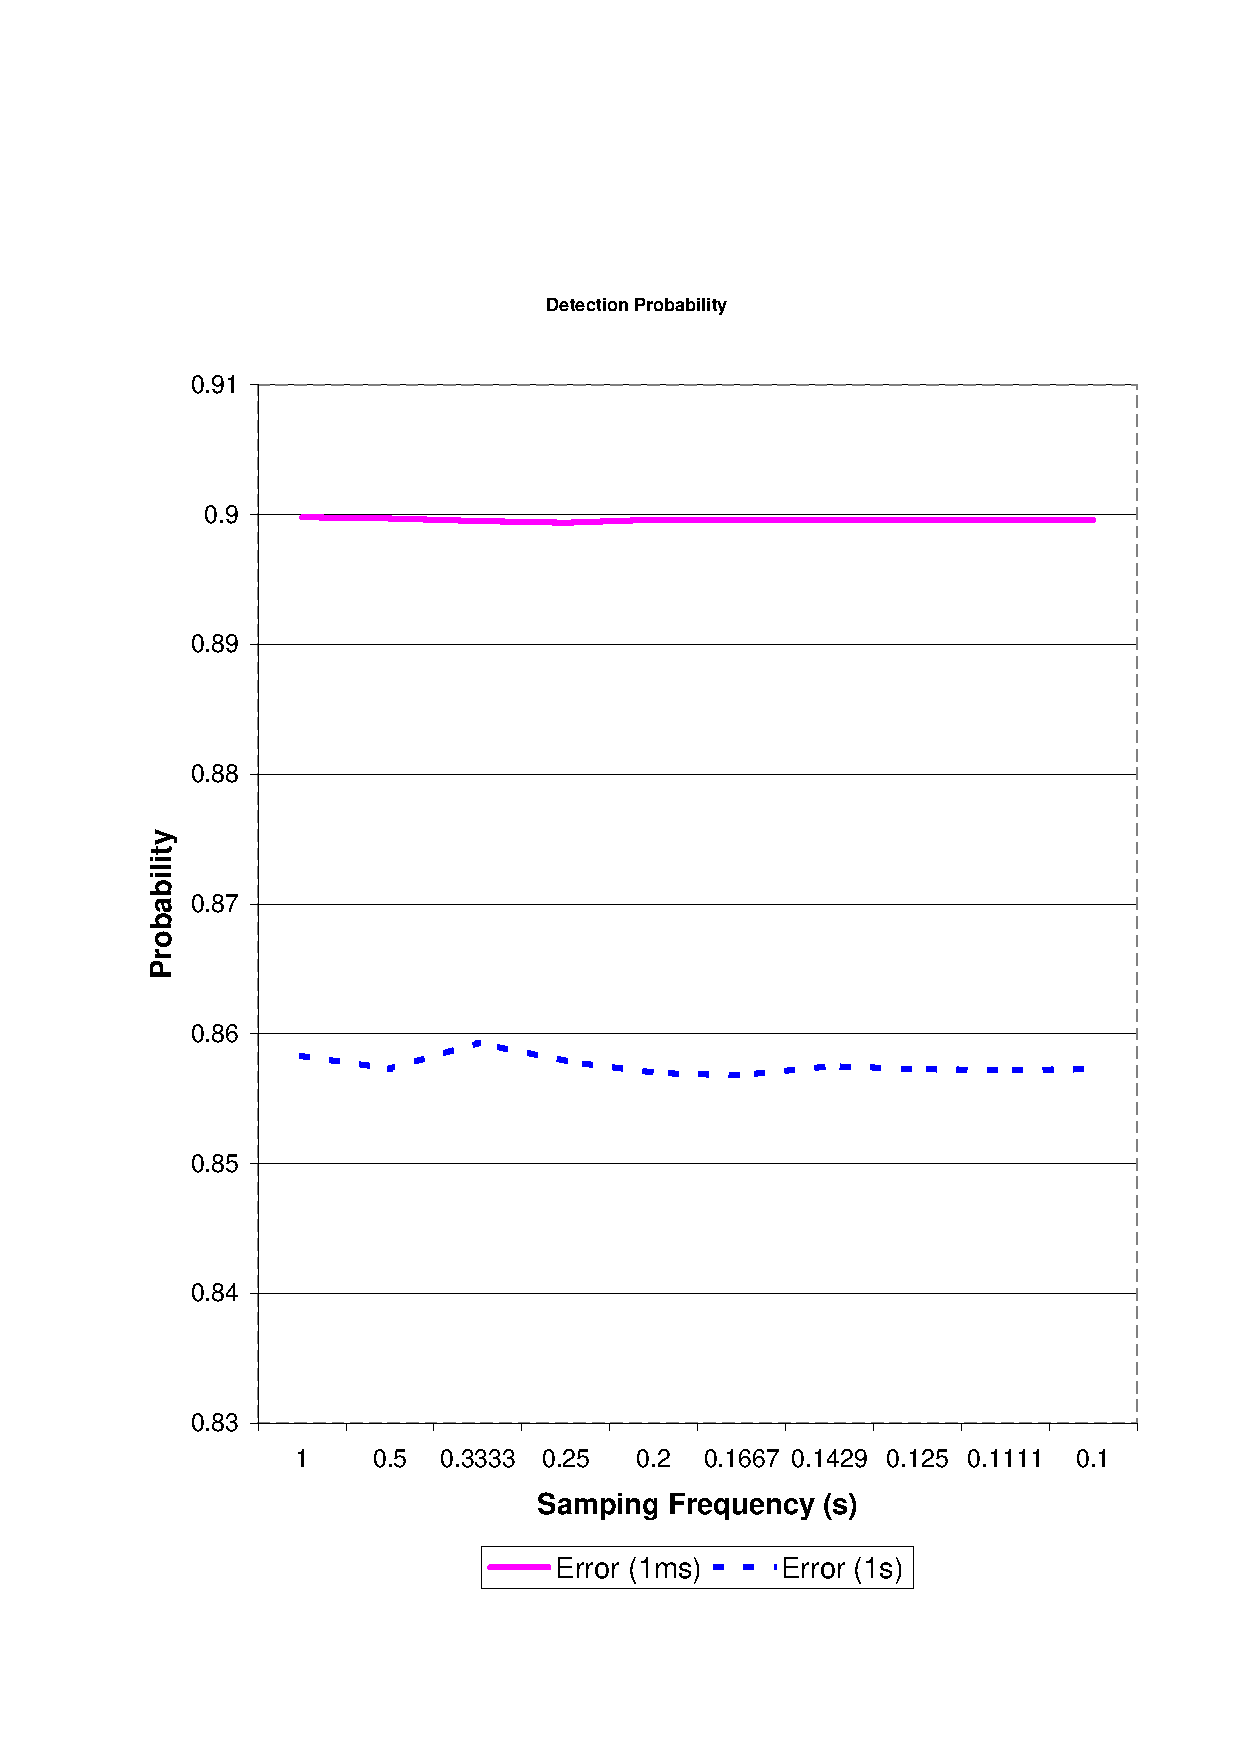
\includegraphics[height=0.3\textheight,width=0.45\textwidth,bbllx=49,bblly=101,bburx=585,bbury=714]{figures/detectionfig}
    \caption{Detection Probability with various sampling frequencies}
        \label{fig:detection}
    \end{center}
\end{figure}
